\pgfdeclareplotmark{cross} {
\pgfpathmoveto{\pgfpoint{-0.3\pgfplotmarksize}{\pgfplotmarksize}}
\pgfpathlineto{\pgfpoint{+0.3\pgfplotmarksize}{\pgfplotmarksize}}
\pgfpathlineto{\pgfpoint{+0.3\pgfplotmarksize}{0.3\pgfplotmarksize}}
\pgfpathlineto{\pgfpoint{+1\pgfplotmarksize}{0.3\pgfplotmarksize}}
\pgfpathlineto{\pgfpoint{+1\pgfplotmarksize}{-0.3\pgfplotmarksize}}
\pgfpathlineto{\pgfpoint{+0.3\pgfplotmarksize}{-0.3\pgfplotmarksize}}
\pgfpathlineto{\pgfpoint{+0.3\pgfplotmarksize}{-1.\pgfplotmarksize}}
\pgfpathlineto{\pgfpoint{-0.3\pgfplotmarksize}{-1.\pgfplotmarksize}}
\pgfpathlineto{\pgfpoint{-0.3\pgfplotmarksize}{-0.3\pgfplotmarksize}}
\pgfpathlineto{\pgfpoint{-1.\pgfplotmarksize}{-0.3\pgfplotmarksize}}
\pgfpathlineto{\pgfpoint{-1.\pgfplotmarksize}{0.3\pgfplotmarksize}}
\pgfpathlineto{\pgfpoint{-0.3\pgfplotmarksize}{0.3\pgfplotmarksize}}
\pgfpathclose
\pgfusepathqstroke
}
\pgfdeclareplotmark{cross*} {
\pgfpathmoveto{\pgfpoint{-0.3\pgfplotmarksize}{\pgfplotmarksize}}
\pgfpathlineto{\pgfpoint{+0.3\pgfplotmarksize}{\pgfplotmarksize}}
\pgfpathlineto{\pgfpoint{+0.3\pgfplotmarksize}{0.3\pgfplotmarksize}}
\pgfpathlineto{\pgfpoint{+1\pgfplotmarksize}{0.3\pgfplotmarksize}}
\pgfpathlineto{\pgfpoint{+1\pgfplotmarksize}{-0.3\pgfplotmarksize}}
\pgfpathlineto{\pgfpoint{+0.3\pgfplotmarksize}{-0.3\pgfplotmarksize}}
\pgfpathlineto{\pgfpoint{+0.3\pgfplotmarksize}{-1.\pgfplotmarksize}}
\pgfpathlineto{\pgfpoint{-0.3\pgfplotmarksize}{-1.\pgfplotmarksize}}
\pgfpathlineto{\pgfpoint{-0.3\pgfplotmarksize}{-0.3\pgfplotmarksize}}
\pgfpathlineto{\pgfpoint{-1.\pgfplotmarksize}{-0.3\pgfplotmarksize}}
\pgfpathlineto{\pgfpoint{-1.\pgfplotmarksize}{0.3\pgfplotmarksize}}
\pgfpathlineto{\pgfpoint{-0.3\pgfplotmarksize}{0.3\pgfplotmarksize}}
\pgfpathclose
\pgfusepathqfillstroke
}
\pgfdeclareplotmark{newstar} {
\pgfpathmoveto{\pgfqpoint{0pt}{\pgfplotmarksize}}
\pgfpathlineto{\pgfqpointpolar{44}{0.5\pgfplotmarksize}}
\pgfpathlineto{\pgfqpointpolar{18}{\pgfplotmarksize}}
\pgfpathlineto{\pgfqpointpolar{-20}{0.5\pgfplotmarksize}}
\pgfpathlineto{\pgfqpointpolar{-54}{\pgfplotmarksize}}
\pgfpathlineto{\pgfqpointpolar{-90}{0.5\pgfplotmarksize}}
\pgfpathlineto{\pgfqpointpolar{234}{\pgfplotmarksize}}
\pgfpathlineto{\pgfqpointpolar{198}{0.5\pgfplotmarksize}}
\pgfpathlineto{\pgfqpointpolar{162}{\pgfplotmarksize}}
\pgfpathlineto{\pgfqpointpolar{134}{0.5\pgfplotmarksize}}
\pgfpathclose
\pgfusepathqstroke
}
\pgfdeclareplotmark{newstar*} {
\pgfpathmoveto{\pgfqpoint{0pt}{\pgfplotmarksize}}
\pgfpathlineto{\pgfqpointpolar{44}{0.5\pgfplotmarksize}}
\pgfpathlineto{\pgfqpointpolar{18}{\pgfplotmarksize}}
\pgfpathlineto{\pgfqpointpolar{-20}{0.5\pgfplotmarksize}}
\pgfpathlineto{\pgfqpointpolar{-54}{\pgfplotmarksize}}
\pgfpathlineto{\pgfqpointpolar{-90}{0.5\pgfplotmarksize}}
\pgfpathlineto{\pgfqpointpolar{234}{\pgfplotmarksize}}
\pgfpathlineto{\pgfqpointpolar{198}{0.5\pgfplotmarksize}}
\pgfpathlineto{\pgfqpointpolar{162}{\pgfplotmarksize}}
\pgfpathlineto{\pgfqpointpolar{134}{0.5\pgfplotmarksize}}
\pgfpathclose
\pgfusepathqfillstroke
}
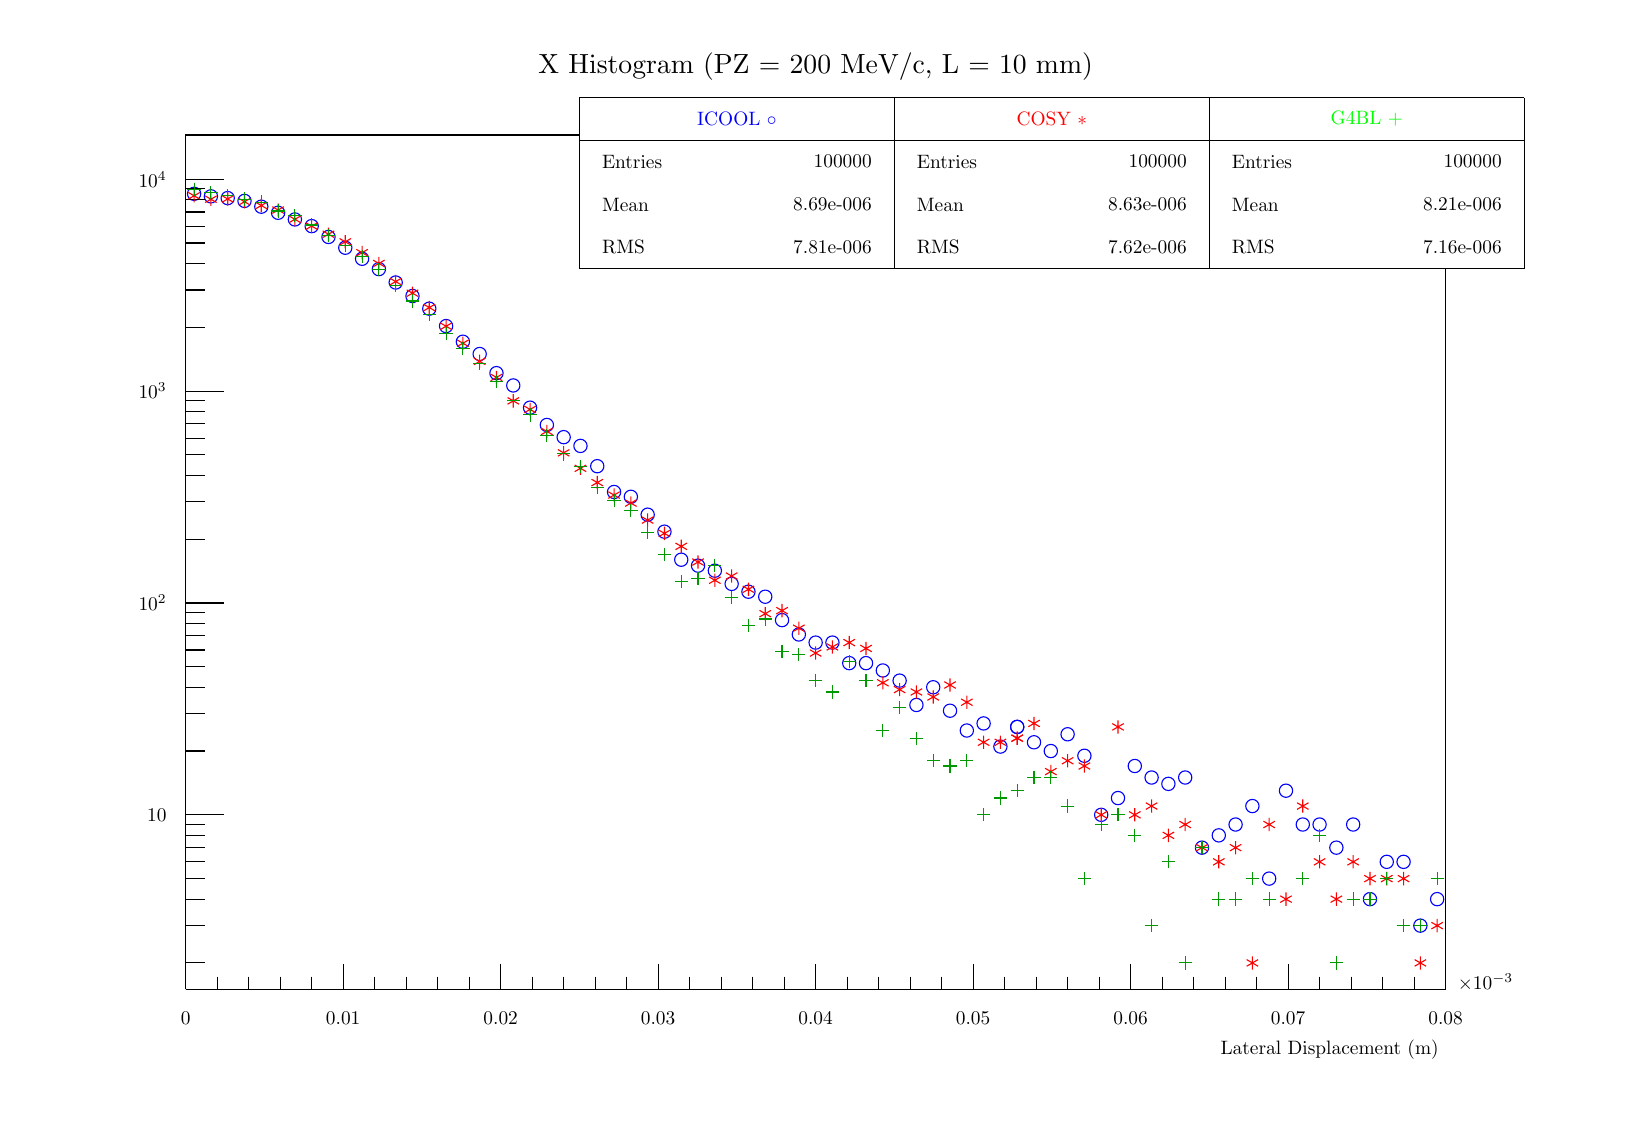
\begin{tikzpicture}
\definecolor{c}{rgb}{1,1,1};
\draw [color=c, fill=c] (0,0) rectangle (20,13.5632);
\draw [color=c, fill=c] (2,1.35632) rectangle (18,12.2069);
\definecolor{c}{rgb}{0,0,0};
\draw [c] (2,1.35632) -- (2,12.2069) -- (18,12.2069) -- (18,1.35632) -- (2,1.35632);
\definecolor{c}{rgb}{1,1,1};
\draw [color=c, fill=c] (2,1.35632) rectangle (18,12.2069);
\definecolor{c}{rgb}{0,0,0};
\draw [c] (2,1.35632) -- (2,12.2069) -- (18,12.2069) -- (18,1.35632) -- (2,1.35632);
\definecolor{c}{rgb}{0,0,1};
\foreach \P in
 {(2.10667,11.4601),(2.32,11.428),(2.53333,11.4057),(2.74667,11.3701),(2.96,11.2967),(3.17333,11.2194),(3.38667,11.1346),(3.6,11.0498),(3.81333,10.9122),(4.02667,10.7755),(4.24,10.635),(4.45333,10.5039),(4.66667,10.3337),(4.88,10.1623),(5.09333,10.00
11),(5.30667,9.78061),(5.52,9.58187),(5.73333,9.42563),(5.94667,9.1825),(6.16,9.02632),(6.37333,8.74419),(6.58667,8.52468),(6.8,8.3696),(7.01333,8.25841),(7.22667,8.00082),(7.44,7.67341),(7.65333,7.61237),(7.86667,7.38521),(8.08,7.16946),(8.29333,6.8
1336),(8.50667,6.73794),(8.72,6.67389),(8.93333,6.50603),(9.14667,6.40694),(9.36,6.34318),(9.57333,6.04637),(9.78667,5.86388),(10,5.7607),(10.2133,5.7607),(10.4267,5.49993),(10.64,5.49993),(10.8533,5.40639),(11.0667,5.27785),(11.28,4.96853),(11.4933,
5.19333),(11.7067,4.89546),(11.92,4.64408),(12.1333,4.73402),(12.3467,4.44033),(12.56,4.68992)}{\draw[mark options={color=c,fill=c},mark size=2.402402pt,mark=o] plot coordinates {\P};}
\foreach \P in
 {(12.56,4.68992),(12.7733,4.4947),(12.9867,4.38332),(13.2,4.59638),(13.4133,4.32338),(13.6267,3.5733),(13.84,3.78636),(14.0533,4.1934),(14.2667,4.04713),(14.48,3.96651),(14.6933,4.04713),(14.9067,3.15649),(15.12,3.31254),(15.3333,3.45018),(15.5467,3
.68468),(15.76,2.76329),(15.9733,3.8799),(16.1867,3.45018),(16.4,3.45018),(16.6133,3.15649),(16.8267,3.45018),(17.04,2.50252),(17.2533,2.97635),(17.4667,2.97635),(17.68,2.16634),(17.8933,2.50252)}{\draw[mark options={color=c,fill=c},mark
 size=2.402402pt,mark=o] plot coordinates {\P};}
\definecolor{c}{rgb}{1,1,1};
\draw [color=c, fill=c] (7,10.5115) rectangle (11,12.6816);
\definecolor{c}{rgb}{0,0,0};
\draw [c] (7,10.5115) -- (11,10.5115);
\draw [c] (11,10.5115) -- (11,12.6816);
\draw [c] (11,12.6816) -- (7,12.6816);
\draw [c] (7,12.6816) -- (7,10.5115);
\draw[color=blue](9,12.4103) node[scale=0.7, rotate=0]{ICOOL $\circ$};
\draw [c] (7,12.1391) -- (11,12.1391);
\draw [anchor= west] (7.2,11.8678) node[scale=0.7, rotate=0]{Entries };
\draw [anchor= east] (10.8,11.8678) node[scale=0.7, rotate=0]{ 100000};
\draw [anchor= west] (7.2,11.3253) node[scale=0.7, rotate=0]{Mean  };
\draw [anchor= east] (10.8,11.3253) node[scale=0.7, rotate=0]{ 8.69e-006};
\draw [anchor= west] (7.2,10.7828) node[scale=0.7, rotate=0]{RMS   };
\draw [anchor= east] (10.8,10.7828) node[scale=0.7, rotate=0]{ 7.81e-006};
\draw [c] (2,1.35632) -- (18,1.35632);
\draw [anchor= east] (18,0.596782) node[scale=0.7, rotate=0]{Lateral Displacement (m)};
\draw [c] (2,1.68184) -- (2,1.35632);
\draw [c] (2.4,1.51908) -- (2.4,1.35632);
\draw [c] (2.8,1.51908) -- (2.8,1.35632);
\draw [c] (3.2,1.51908) -- (3.2,1.35632);
\draw [c] (3.6,1.51908) -- (3.6,1.35632);
\draw [c] (4,1.68184) -- (4,1.35632);
\draw [c] (4.4,1.51908) -- (4.4,1.35632);
\draw [c] (4.8,1.51908) -- (4.8,1.35632);
\draw [c] (5.2,1.51908) -- (5.2,1.35632);
\draw [c] (5.6,1.51908) -- (5.6,1.35632);
\draw [c] (6,1.68184) -- (6,1.35632);
\draw [c] (6.4,1.51908) -- (6.4,1.35632);
\draw [c] (6.8,1.51908) -- (6.8,1.35632);
\draw [c] (7.2,1.51908) -- (7.2,1.35632);
\draw [c] (7.6,1.51908) -- (7.6,1.35632);
\draw [c] (8,1.68184) -- (8,1.35632);
\draw [c] (8.4,1.51908) -- (8.4,1.35632);
\draw [c] (8.8,1.51908) -- (8.8,1.35632);
\draw [c] (9.2,1.51908) -- (9.2,1.35632);
\draw [c] (9.6,1.51908) -- (9.6,1.35632);
\draw [c] (10,1.68184) -- (10,1.35632);
\draw [c] (10.4,1.51908) -- (10.4,1.35632);
\draw [c] (10.8,1.51908) -- (10.8,1.35632);
\draw [c] (11.2,1.51908) -- (11.2,1.35632);
\draw [c] (11.6,1.51908) -- (11.6,1.35632);
\draw [c] (12,1.68184) -- (12,1.35632);
\draw [c] (12.4,1.51908) -- (12.4,1.35632);
\draw [c] (12.8,1.51908) -- (12.8,1.35632);
\draw [c] (13.2,1.51908) -- (13.2,1.35632);
\draw [c] (13.6,1.51908) -- (13.6,1.35632);
\draw [c] (14,1.68184) -- (14,1.35632);
\draw [c] (14.4,1.51908) -- (14.4,1.35632);
\draw [c] (14.8,1.51908) -- (14.8,1.35632);
\draw [c] (15.2,1.51908) -- (15.2,1.35632);
\draw [c] (15.6,1.51908) -- (15.6,1.35632);
\draw [c] (16,1.68184) -- (16,1.35632);
\draw [c] (16.4,1.51908) -- (16.4,1.35632);
\draw [c] (16.8,1.51908) -- (16.8,1.35632);
\draw [c] (17.2,1.51908) -- (17.2,1.35632);
\draw [c] (17.6,1.51908) -- (17.6,1.35632);
\draw [c] (18,1.68184) -- (18,1.35632);
\draw [c] (18,1.68184) -- (18,1.35632);
\draw [anchor=base] (2,0.908736) node[scale=0.7, rotate=0]{0};
\draw [anchor=base] (4,0.908736) node[scale=0.7, rotate=0]{0.01};
\draw [anchor=base] (6,0.908736) node[scale=0.7, rotate=0]{0.02};
\draw [anchor=base] (8,0.908736) node[scale=0.7, rotate=0]{0.03};
\draw [anchor=base] (10,0.908736) node[scale=0.7, rotate=0]{0.04};
\draw [anchor=base] (12,0.908736) node[scale=0.7, rotate=0]{0.05};
\draw [anchor=base] (14,0.908736) node[scale=0.7, rotate=0]{0.06};
\draw [anchor=base] (16,0.908736) node[scale=0.7, rotate=0]{0.07};
\draw [anchor=base] (18,0.908736) node[scale=0.7, rotate=0]{0.08};
\draw [anchor=base west] (18.07,1.35632) node[scale=0.7, rotate=0]{$\times10^{-3}$};
\draw [c] (2,1.35632) -- (2,12.2069);
\draw [c] (2.24,1.69251) -- (2,1.69251);
\draw [c] (2.24,2.16633) -- (2,2.16633);
\draw [c] (2.24,2.50252) -- (2,2.50252);
\draw [c] (2.24,2.76329) -- (2,2.76329);
\draw [c] (2.24,2.97635) -- (2,2.97635);
\draw [c] (2.24,3.15649) -- (2,3.15649);
\draw [c] (2.24,3.31253) -- (2,3.31253);
\draw [c] (2.24,3.45018) -- (2,3.45018);
\draw [c] (2.48,3.5733) -- (2,3.5733);
\draw [anchor= east] (1.844,3.5733) node[scale=0.7, rotate=0]{10};
\draw [c] (2.24,4.38332) -- (2,4.38332);
\draw [c] (2.24,4.85714) -- (2,4.85714);
\draw [c] (2.24,5.19333) -- (2,5.19333);
\draw [c] (2.24,5.4541) -- (2,5.4541);
\draw [c] (2.24,5.66716) -- (2,5.66716);
\draw [c] (2.24,5.8473) -- (2,5.8473);
\draw [c] (2.24,6.00334) -- (2,6.00334);
\draw [c] (2.24,6.14099) -- (2,6.14099);
\draw [c] (2.48,6.26411) -- (2,6.26411);
\draw [anchor= east] (1.844,6.26411) node[scale=0.7, rotate=0]{$10^{2}$};
\draw [c] (2.24,7.07413) -- (2,7.07413);
\draw [c] (2.24,7.54795) -- (2,7.54795);
\draw [c] (2.24,7.88414) -- (2,7.88414);
\draw [c] (2.24,8.14491) -- (2,8.14491);
\draw [c] (2.24,8.35797) -- (2,8.35797);
\draw [c] (2.24,8.53811) -- (2,8.53811);
\draw [c] (2.24,8.69415) -- (2,8.69415);
\draw [c] (2.24,8.8318) -- (2,8.8318);
\draw [c] (2.48,8.95492) -- (2,8.95492);
\draw [anchor= east] (1.844,8.95492) node[scale=0.7, rotate=0]{$10^{3}$};
\draw [c] (2.24,9.76494) -- (2,9.76494);
\draw [c] (2.24,10.2388) -- (2,10.2388);
\draw [c] (2.24,10.575) -- (2,10.575);
\draw [c] (2.24,10.8357) -- (2,10.8357);
\draw [c] (2.24,11.0488) -- (2,11.0488);
\draw [c] (2.24,11.2289) -- (2,11.2289);
\draw [c] (2.24,11.385) -- (2,11.385);
\draw [c] (2.24,11.5226) -- (2,11.5226);
\draw [c] (2.48,11.6457) -- (2,11.6457);
\draw [anchor= east] (1.844,11.6457) node[scale=0.7, rotate=0]{$10^{4}$};
\definecolor{c}{rgb}{1,1,1};
\draw [color=c, fill=c] (7,10.5115) rectangle (11,12.6816);
\definecolor{c}{rgb}{0,0,0};
\draw [c] (7,10.5115) -- (11,10.5115);
\draw [c] (11,10.5115) -- (11,12.6816);
\draw [c] (11,12.6816) -- (7,12.6816);
\draw [c] (7,12.6816) -- (7,10.5115);
\draw[color=blue](9,12.4103) node[scale=0.7, rotate=0]{ICOOL $\circ$};
\draw [c] (7,12.1391) -- (11,12.1391);
\draw [anchor= west] (7.2,11.8678) node[scale=0.7, rotate=0]{Entries };
\draw [anchor= east] (10.8,11.8678) node[scale=0.7, rotate=0]{ 100000};
\draw [anchor= west] (7.2,11.3253) node[scale=0.7, rotate=0]{Mean  };
\draw [anchor= east] (10.8,11.3253) node[scale=0.7, rotate=0]{ 8.69e-006};
\draw [anchor= west] (7.2,10.7828) node[scale=0.7, rotate=0]{RMS   };
\draw [anchor= east] (10.8,10.7828) node[scale=0.7, rotate=0]{ 7.81e-006};
\draw (10,13.0816) node[scale=1, rotate=0]{X Histogram (PZ = 200 MeV/c, L = 10 mm)};
\definecolor{c}{rgb}{1,0,0};
\foreach \P in
 {(2.10667,11.4351),(2.32,11.3914),(2.53333,11.3947),(2.74667,11.3596),(2.96,11.3116),(3.17333,11.2542),(3.38667,11.1362),(3.6,11.0499),(3.81333,10.9469),(4.02667,10.8506),(4.24,10.7129),(4.45333,10.5755),(4.66667,10.3455),(4.88,10.1983),(5.09333,10.
0154),(5.30667,9.7783),(5.52,9.56258),(5.73333,9.33216),(5.94667,9.12837),(6.16,8.8305),(6.37333,8.72159),(6.58667,8.44248),(6.8,8.17034),(7.01333,7.97408),(7.22667,7.79304),(7.44,7.63428),(7.65333,7.53227),(7.86667,7.31604),(8.08,7.14772),(8.29333,6
.98302),(8.50667,6.78377),(8.72,6.55259),(8.93333,6.60613),(9.14667,6.43756),(9.36,6.12793),(9.57333,6.16667),(9.78667,5.9434),(10,5.62754),(10.2133,5.70548),(10.4267,5.7607),(10.64,5.68648),(10.8533,5.25035),(11.0667,5.16375),(11.28,5.13339),(11.493
3,5.07021),(11.7067,5.22219),(11.92,5.00341),(12.1333,4.4947),(12.3467,4.4947),(12.56,4.54664)}{\draw[mark options={color=c,fill=c},mark size=2.402402pt,mark=asterisk] plot coordinates {\P};}
\foreach \P in
 {(12.56,4.54664),(12.7733,4.73402),(12.9867,4.12255),(13.2,4.26019),(13.4133,4.1934),(13.6267,3.5733),(13.84,4.68992),(14.0533,3.5733),(14.2667,3.68468),(14.48,3.31254),(14.6933,3.45018),(14.9067,3.15649),(15.12,2.97635),(15.3333,3.15649),(15.5467,1
.69251),(15.76,3.45018),(15.9733,2.50252),(16.1867,3.68468),(16.4,2.97635),(16.6133,2.50252),(16.8267,2.97635),(17.04,2.76329),(17.2533,2.76329),(17.4667,2.76329),(17.68,1.69251),(17.8933,2.16634)}{\draw[mark options={color=c,fill=c},mark
 size=2.402402pt,mark=asterisk] plot coordinates {\P};}
\definecolor{c}{rgb}{1,1,1};
\draw [color=c, fill=c] (11,10.5115) rectangle (15,12.6816);
\definecolor{c}{rgb}{0,0,0};
\draw [c] (11,10.5115) -- (15,10.5115);
\draw [c] (15,10.5115) -- (15,12.6816);
\draw [c] (15,12.6816) -- (11,12.6816);
\draw [c] (11,12.6816) -- (11,10.5115);
\draw [color=red](13,12.4103) node[scale=0.7, rotate=0]{COSY $*$};
\draw [c] (11,12.1391) -- (15,12.1391);
\draw [anchor= west] (11.2,11.8678) node[scale=0.7, rotate=0]{Entries };
\draw [anchor= east] (14.8,11.8678) node[scale=0.7, rotate=0]{ 100000};
\draw [anchor= west] (11.2,11.3253) node[scale=0.7, rotate=0]{Mean  };
\draw [anchor= east] (14.8,11.3253) node[scale=0.7, rotate=0]{ 8.63e-006};
\draw [anchor= west] (11.2,10.7828) node[scale=0.7, rotate=0]{RMS   };
\draw [anchor= east] (14.8,10.7828) node[scale=0.7, rotate=0]{ 7.62e-006};
\definecolor{c}{rgb}{1,1,1};
\draw [color=c, fill=c] (11,10.5115) rectangle (15,12.6816);
\definecolor{c}{rgb}{0,0,0};
\draw [c] (11,10.5115) -- (15,10.5115);
\draw [c] (15,10.5115) -- (15,12.6816);
\draw [c] (15,12.6816) -- (11,12.6816);
\draw [c] (11,12.6816) -- (11,10.5115);
\draw [color=red](13,12.4103) node[scale=0.7, rotate=0]{COSY $*$};
\draw [c] (11,12.1391) -- (15,12.1391);
\draw [anchor= west] (11.2,11.8678) node[scale=0.7, rotate=0]{Entries };
\draw [anchor= east] (14.8,11.8678) node[scale=0.7, rotate=0]{ 100000};
\draw [anchor= west] (11.2,11.3253) node[scale=0.7, rotate=0]{Mean  };
\draw [anchor= east] (14.8,11.3253) node[scale=0.7, rotate=0]{ 8.63e-006};
\draw [anchor= west] (11.2,10.7828) node[scale=0.7, rotate=0]{RMS   };
\draw [anchor= east] (14.8,10.7828) node[scale=0.7, rotate=0]{ 7.62e-006};
\definecolor{c}{rgb}{0,0.6,0};
\foreach \P in
 {(2.10667,11.5173),(2.32,11.4767),(2.53333,11.4342),(2.74667,11.3931),(2.96,11.3543),(3.17333,11.242),(3.38667,11.1828),(3.6,11.0635),(3.81333,10.9304),(4.02667,10.8018),(4.24,10.6603),(4.45333,10.4952),(4.66667,10.2999),(4.88,10.0991),(5.09333,9.92
877),(5.30667,9.68952),(5.52,9.4939),(5.73333,9.30649),(5.94667,9.07688),(6.16,8.83439),(6.37333,8.65252),(6.58667,8.39062),(6.8,8.15654),(7.01333,7.99552),(7.22667,7.7281),(7.44,7.56343),(7.65333,7.43774),(7.86667,7.16406),(8.08,6.87731),(8.29333,6.
53419),(8.50667,6.57071),(8.72,6.73794),(8.93333,6.33221),(9.14667,5.97376),(9.36,6.06036),(9.57333,5.64752),(9.78667,5.60722),(10,5.27785),(10.2133,5.13339),(10.4267,5.52219),(10.64,5.27785),(10.8533,4.64408),(11.0667,4.93257),(11.28,4.54664),(11.49
33,4.26019),(11.7067,4.1934),(11.92,4.26019),(12.1333,3.5733),(12.3467,3.78636),(12.56,3.8799)}{\draw[mark options={color=c,fill=c},mark size=2.402402pt,mark=+] plot coordinates {\P};}
\foreach \P in
 {(12.56,3.8799),(12.7733,4.04713),(12.9867,4.04713),(13.2,3.68468),(13.4133,2.76329),(13.6267,3.45018),(13.84,3.5733),(14.0533,3.31254),(14.2667,2.16634),(14.48,2.97635),(14.6933,1.69251),(14.9067,3.15649),(15.12,2.50252),(15.3333,2.50252),(15.5467,
2.76329),(15.76,2.50252),(16.1867,2.76329),(16.4,3.31254),(16.6133,1.69251),(16.8267,2.50252),(17.04,2.50252),(17.2533,2.76329),(17.4667,2.16634),(17.68,2.16634),(17.8933,2.76329)}{\draw[mark options={color=c,fill=c},mark size=2.402402pt,mark=+] plot
 coordinates {\P};}
\definecolor{c}{rgb}{1,1,1};
\draw [color=c, fill=c] (15,10.5115) rectangle (19,12.6816);
\definecolor{c}{rgb}{0,0,0};
\draw [c] (15,10.5115) -- (19,10.5115);
\draw [c] (19,10.5115) -- (19,12.6816);
\draw [c] (19,12.6816) -- (15,12.6816);
\draw [c] (15,12.6816) -- (15,10.5115);
\draw [color=green](17,12.4103) node[scale=0.7, rotate=0]{G4BL $+$};
\draw [c] (15,12.1391) -- (19,12.1391);
\draw [anchor= west] (15.2,11.8678) node[scale=0.7, rotate=0]{Entries };
\draw [anchor= east] (18.8,11.8678) node[scale=0.7, rotate=0]{ 100000};
\draw [anchor= west] (15.2,11.3253) node[scale=0.7, rotate=0]{Mean  };
\draw [anchor= east] (18.8,11.3253) node[scale=0.7, rotate=0]{ 8.21e-006};
\draw [anchor= west] (15.2,10.7828) node[scale=0.7, rotate=0]{RMS   };
\draw [anchor= east] (18.8,10.7828) node[scale=0.7, rotate=0]{ 7.16e-006};
\definecolor{c}{rgb}{1,1,1};
\draw [color=c, fill=c] (15,10.5115) rectangle (19,12.6816);
\definecolor{c}{rgb}{0,0,0};
\draw [c] (15,10.5115) -- (19,10.5115);
\draw [c] (19,10.5115) -- (19,12.6816);
\draw [c] (19,12.6816) -- (15,12.6816);
\draw [c] (15,12.6816) -- (15,10.5115);
\draw [color=green](17,12.4103) node[scale=0.7, rotate=0]{G4BL $+$};
\draw [c] (15,12.1391) -- (19,12.1391);
\draw [anchor= west] (15.2,11.8678) node[scale=0.7, rotate=0]{Entries };
\draw [anchor= east] (18.8,11.8678) node[scale=0.7, rotate=0]{ 100000};
\draw [anchor= west] (15.2,11.3253) node[scale=0.7, rotate=0]{Mean  };
\draw [anchor= east] (18.8,11.3253) node[scale=0.7, rotate=0]{ 8.21e-006};
\draw [anchor= west] (15.2,10.7828) node[scale=0.7, rotate=0]{RMS   };
\draw [anchor= east] (18.8,10.7828) node[scale=0.7, rotate=0]{ 7.16e-006};
\end{tikzpicture}
